\documentclass[10pt]{beamer}
\usetheme{metropolis}           % Use metropolis theme
\usepackage[utf8]{inputenc}
\usepackage{amsmath,amsfonts,amssymb}
\usepackage{dsfont}
\usepackage{graphicx}
\usepackage{caption}
\usefonttheme[onlymath]{serif}


\title{Difféomorphismes du cercle et théorème de Nash-Moser}
\date{14 Mai 2024}
\author{Sacha Ben-Arous, Mathis Bordet}
\institute{ENS Paris-Saclay}
\begin{document}
  \maketitle
\begin{frame}
\tableofcontents
\end{frame}  



\section{Difféomorphismes du cercle}
\begin{frame}{Dynamique en dimension 1}
    On considère le cercle $\mathbb{S}^1 := \left\{z, |z|=1 \right\}$, ainsi que le plongement $\Pi : \mathbb{R} \mapsto \mathbb{S}^1, t \mapsto e^{2i\pi t}$. \\
    
Pour $f:\mathbb{S}^1 \mapsto \mathbb{S}^1$, on dit que $F: \mathbb{R} \mapsto \mathbb{R}$ est un relèvement si $\Pi \circ F = f \circ \Pi$, i.e $f(e^{2i\pi t}) = e^{2i\pi F(t)}$

\textbf{Lemme :} Si $f$ est un $\mathcal{C}^k$-difféomorphisme du cercle, alors il existe un relèvement de $f$ qui est un $\mathcal{C}^k$-difféomorphisme (de $\mathbb{R}$). \\~\\

Dans la suite, on considèrera a minima des homéomorphismes, ainsi que leur relèvements réguliers associés.
\end{frame}

\begin{frame}{Nombre de rotation}
    Si $f$ est un homéomorphisme, $F$ un relèvement, et $x\in \mathbb{R}$, la suite $\displaystyle (\frac{F^n(x)}{n})_{n\in \mathbb{N}}$ converge vers une limite indépendante de $x$, notée $\rho(F)$. On définit alors $\rho(f):= \rho(F) \mod 1$. \\~\\
    
$\rho$ n'est \textbf{pas} un morphisme, mais vérifie $\rho(h\circ f \circ h^{-1}) = \rho(f)$, c'est un invariant de conjuguaison. \\~\\

On se demande alors si il existe un représentant simple de la classe de $f$, à savoir $R_{\rho(f)}$.
\end{frame}



\begin{frame}{Théorème de Poincaré}
Le résultat est clairement faux quand $\rho(f) \in \mathbb{Q}$. Dans le cas irrationnel, on a le résultat suivant : \\~\\

\textbf{Théorème (Poincaré) :} Si $f$ est un homéomorphisme de nombre de rotation $\alpha$ irrationnel, alors $f$ est semi-conjugué à $R_\alpha$, i.e il existe $h$ continue telle que $h \circ f = R_\alpha \circ h$. \\~\\

Que dire de l'inversibilité de $h$ ?
\end{frame}


\begin{frame}{Théorème de Denjoy}
\textbf{Théorème (Denjoy) :} Si $f$ est un $\mathcal{C}^2$-difféomorphisme de nombre de rotation $\alpha$ irrationnel, alors $f$ est conjugué à $R_\alpha$ par un homéomorphisme. \\~\\

\underline{Idée de la preuve }: Il ne peut pas exister d'intervalle errant pour $h$. \\~\\

\underline{Question }: Le résultat est-il optimal ?

\end{frame}


\begin{frame}{Contre-exemples}
\textbf{Théorème (Herman) :} Pour tout $\alpha$ irrationnel, $\forall \epsilon > 0$, il existe un $\mathcal{C}^{2-\epsilon}$-difféomorphisme $f$ tel que $\rho(f)=\alpha$ et $f$ n'est pas conjugué à la rotation $R_\alpha$. Ces contre-exemples sont de plus denses dans l'ensemble des difféomorphismes de nombre de rotation $\alpha$. \\~\\

\underline{Idée }: Un homéomorphisme $f$ est dit \textit{minimal} si tout ensemble fermé invariant par  $f$ est vide ou égal au cercle tout entier. Cette propriété est un invariant de conjuguaison.
\end{frame}



\begin{frame}{Construction explicite}

\begin{centering}
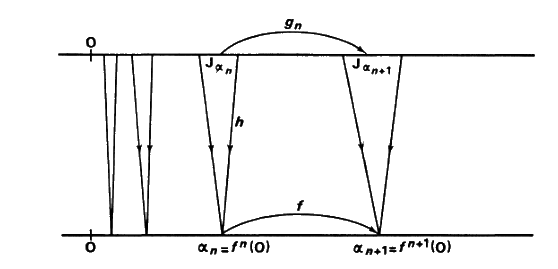
\includegraphics[scale=0.35]{diagram.png}
\captionof{figure}{Schéma de la construction où $f=R_\alpha$}
\end{centering}

On construit un difféo non minimal mais suffisamment régulier en choisissant judicieusement la famille d'intervalles errants.
\end{frame}

\section{Théorème d'Arnold}
\begin{frame}
\frametitle{Cadre}
Prenons un relevé $F$ analytique de rotation $\alpha$ (et donc semi-conjugué à $R_\alpha$). Que l'on écrit :
\[ F(x) = x + \alpha + \eta (x) \]
avec $\eta$ analytique et "assez petit".

$\eta$ est également 1-périodique.
\end{frame}

\begin{frame}
\frametitle{Détermination}
Par théorème de semi-conjugaison, on a :
\[ F \circ H(x) = H( x + \alpha) \text{ et on cherche } H \text{ de la forme } H = \text{id} + U \]
\[ \Rightarrow U(x+ \alpha) - U(x) = \eta (x+U(x)) \text{ simplifié en } U(x+ \alpha) - U(x) = \eta (x) \]
On choisit de chercher \( U \) 1-périodique. On a que 
\[ (\exp(2 i \pi n \alpha)-1)\widehat{U} (n) = \widehat{\eta} (n) \]
\end{frame}

\begin{frame}
\frametitle{Perte de régularité et petits diviseurs}
Dans quelle mesure \( \widehat{U} \) est-elle liée à une série de Fourier convergente ?

En effet, \( \exp(2 i \pi n \alpha)-1 \) peut arbitrairement s'approcher de 0.

Petit diviseur avec \( \alpha \) irrationnel: \( \left\| \alpha - \frac{m}{n} \right\| \geq \frac{k}{n^\nu} \Rightarrow \left\| \exp(2 i \pi n \alpha)-1\right\| \geq \frac{4k}{n^{\nu-1}} \)

Induit la perte de régularité suivante
\[
\begin{aligned}
& \|F\|{H{\text{per}}^s} = \left(\sum_{n \in \mathbb{Z}}|n|^{2 s}|\hat{F}(n)|^2\right)^{1 / 2}, \quad s \geq 0 \\
& \|U\|{H{\text{per}}^s} \leq \frac{1}{4 K}\|\eta\|{H{\text{per}}^{s+\nu-1}} .
\end{aligned}
\]
\end{frame}

\begin{frame}
\frametitle{Enoncé et Preuve}
Le théorème d'Arnold affirme donc que si \( F \) a un relevé \( F(x) = x + \alpha + \eta (x) \) avec \( \eta \) analytique et assez petit (au sens d'une norme analytique), alors \( F \) est analytiquement conjugué à \( R_\alpha \).

Éléments de démonstration :
\begin{itemize}
    \item \( U_n \) la solution de \( U_n(x+\alpha)-U_n(x)=\eta_n(x)-\hat{\eta}_n(0) \).
    \item \( H_n(x)=x+U_n(x) \).
    \item \( F_{n+1}=H_n^{-1} \circ F_n \circ H_n=\left(H_1 \circ \cdots \circ H_n\right)^{-1} \circ F \circ\left(H_1 \circ \cdots \circ H_n\right) \).
\end{itemize}
\end{frame}
\section{Théorème de Nash-Moser}
\begin{frame}
\frametitle{Cadre}
On considère ici deux suites d'espaces de Banach ${E}\sigma, \lVert \cdot \rVert\sigma$ et ${F}\sigma, \lVert \cdot \rVert\sigma$.

De telle sorte qu'il existe une fonction régularisante $S$ telle que 
\[
\forall \theta \in \mathbb{R}, \quad S : E \to F 
\]

\begin{enumerate}
    \item $\left\|S_\theta u\right\|_b \leq C\|u\|_a$, si $b \leq a$
    \item $\left\|S_\theta u\right\|_b \leq C \theta^{b-a}\|u\|_a$, si $a < b$
    \item $\left\|u-S_\theta u\right\|_b \leq C \theta^{b-a}\|u\|_a$, si $a > b$
    \item $\left\|\frac{d}{d \theta} S_\theta u\right\|_b \leq C \theta^{b-a-1}\|u\|_a$.
\end{enumerate}
\end{frame}

\begin{frame}
\frametitle{Enoncé }
Soit $a_2 \in \mathbf{R}$ et soit $\alpha , \beta \in [0;a_2 ]$.
De plus, considérons une application $\Phi : E_\alpha \to F_\beta \: C^2 $ vérifiant :
\[ \left\|\Phi '' (u)(v,w) \right\|{\beta + \delta} \leq C ( 1 +\left\|u \right\|\alpha ) \left\|w \right\|{\alpha - \frac{\epsilon}{2} } \cdot \left\| v \right\|{\alpha - \frac{\epsilon}{2}} \]  
On a de plus l'existence d'une inverse à droite pour $\Phi' $, c'est-à-dire :
$\forall v \in E_\infty$, on a $\Psi (v): f_\infty \to E_\infty $ avec 
\[ \left\| \Psi(v)g \right\|a \leq C \left\| g \right\|{\beta + a - \alpha }+ \left\| g \right\|0 \left\| v \right\|{\alpha + \beta} \]
Alors, $\exists \eta > 0 $ telle que $\forall f \in F_\beta$ vérifiant $ \left\| f \right\|\beta \leq \eta$, alors $\exists u \in E\alpha$ vérifiant $ \Phi(u)-\Phi(0)=f$.
\end{frame}

\begin{frame}
\frametitle{Outil}
On prend $\theta_j$ une suite d'indices divergents et on définit $\Delta_j= \theta_{j+1} - \theta_{j}$ et $R_j u=\left(S_{\theta_{j+1}} u-S_{\theta_j} u\right) / \Delta_j$ si $j>0$, $R_0 u=S_{\theta_1} u / \Delta_0$.

On obtient alors :
\[ u=\sum_{j=0}^{\infty} \Delta_j R_j u \]
Convergente dans $E_a$ si $u \in E_b$ et $a < b$.
\end{frame}

\begin{frame}
\frametitle{Schéma de la preuve:}
On construit les suites suivantes en prenant g $\in F_\beta$
$$
g=\sum \Delta_j g_j ; \quad\left\|g_j\right\|b \leqq C_b \theta_j^{b-\beta-1}\|g\|\beta^{\prime} .
$$
$$
u_{j+1}=u_j+\Delta_j \dot{u}j, \quad \dot{u}_j=\psi\left(v_j\right) g_j, \quad v_j=S{\theta_j} u_j
$$
et on montre que $\Phi(u) -\Phi(0) = T(g) + g$ avec T application continue . 
\end{frame}



\begin{frame}{Fin}

\begin{center}
Merci pour votre attention ! \\~\\
Q\&A
\end{center}

\end{frame}

\end{document}

